Contemporary language models are remarkably proficient on a wide range of natural language tasks \citep{brown2020language,ouyang2022training,touvron2023llama,achiam2023gpt,anil2023palm},  
but inherit shortcomings of the data on which they were trained. 
A fundamental challenge is to achieve better performance than what is directly induced by the distribution of available, human-generated training data. To this end, recent
work
\citep{huang2022large,wang2022self,bai2022constitutional,pang2023language,yuan2024self}
has raised the possibility of ``self-improvement,'' where a
model---typically through forms of self-play or self-training in which the
model critiques its own generations---learns to improve on its own,
without external feedback. This phenomenon is somewhat counterintuitive; at first glance it would seem to
disagree with the well-known data-processing inequality
\citep{cover1999elements}, which implies that no form of self-training
should be able to create information not already in the
model. This motivates the question of why we should expect such supervision-free interventions will lead to
stronger reasoning and planning capabilities.\loose%





  A dominant hypothesis for why improvement without external feedback might be possible is that 
  models contain ``hidden knowledge''~\citep{hinton2015distilling} that 
  is difficult to access. Self-improvement, rather than creating knowledge 
  from nothing, is a means of extracting and distilling this knowledge into a more
  accessible form, and thus is a computational
  phenomenon rather than a statistical one. 
  While there is a growing body of empirical evidence for this
  hidden-knowledge hypothesis
  \citep{furlanello2018born,gotmare2019closer,dong2019distillation,abnar2020transferring,allen2020towards},
  particularly in the context of self-distillation, a fundamental understanding of self-improvement remains missing. Concretely, where in the model is this hidden knowledge, and when and how can it be extracted? \loose







        

  \subsection{Our Perspective: The Sharpening Mechanism}

\begin{figure}[t]
    \centering
    \subfigure[]{
        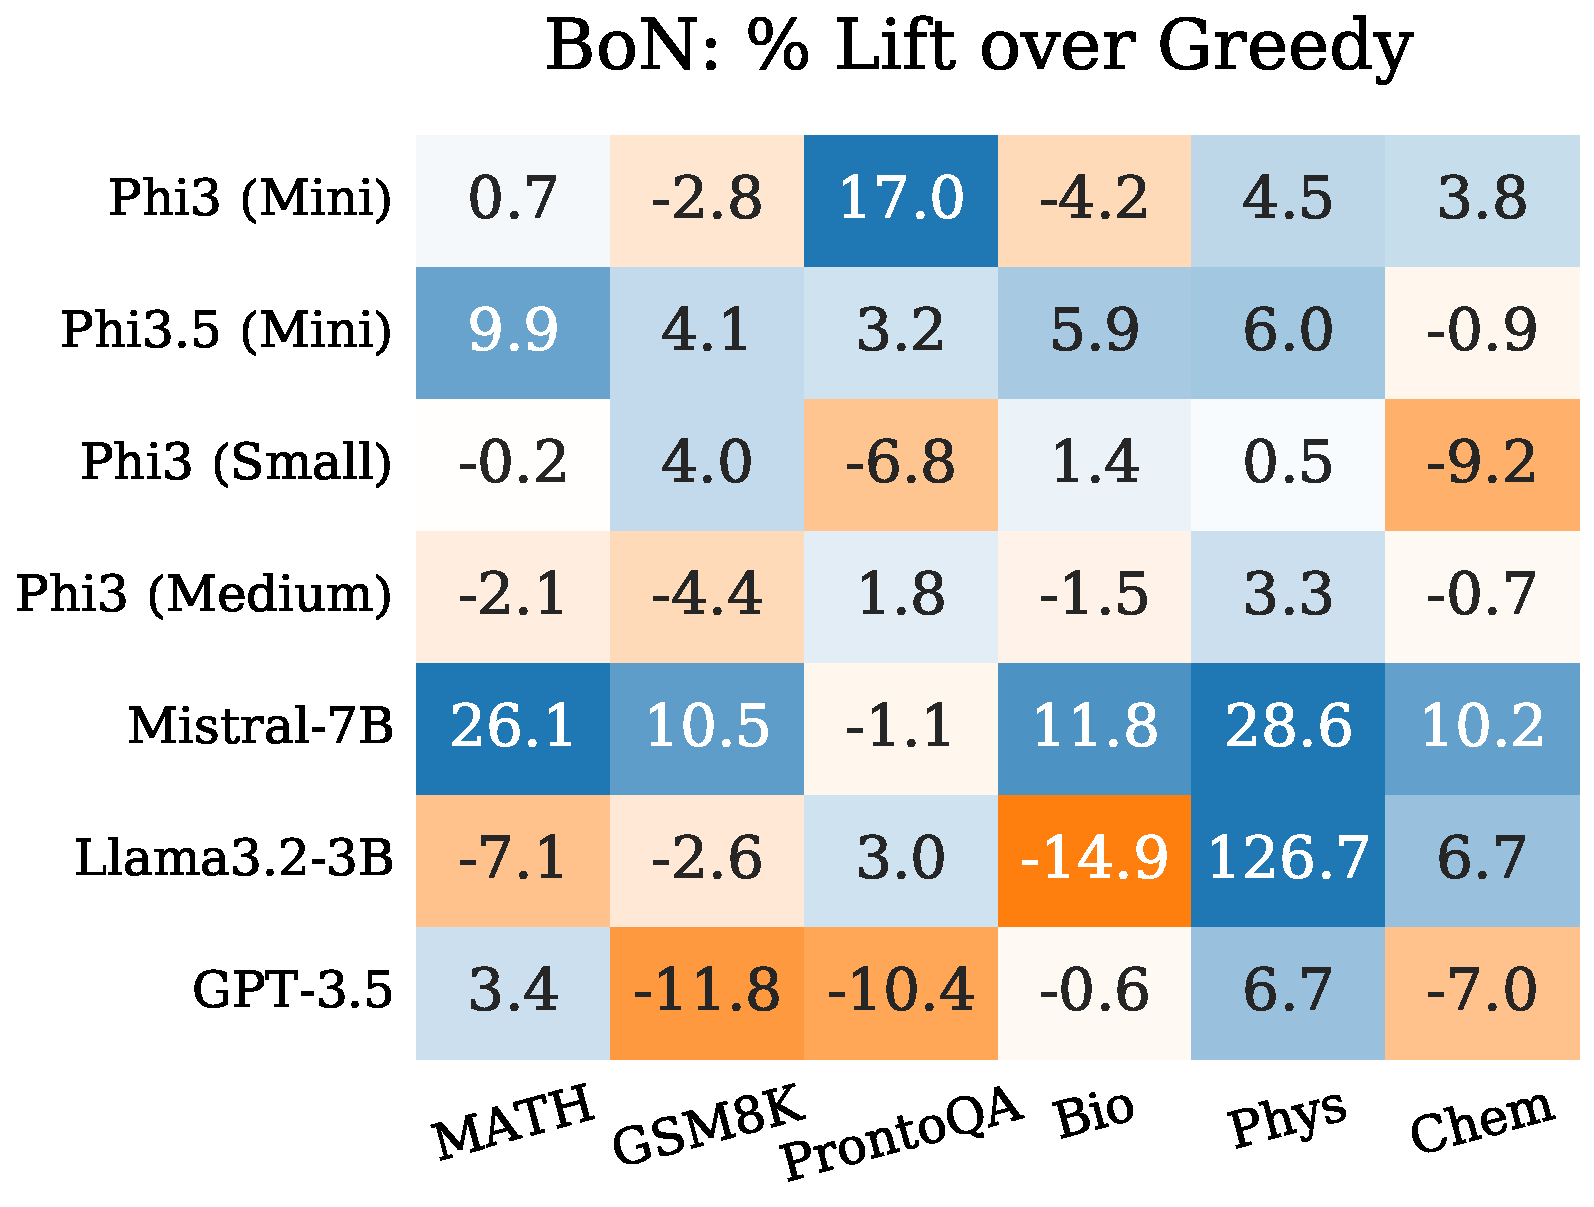
\includegraphics[width=0.32\textwidth]{figs/Fig-1-BoN-Colored-Table.pdf}
        \label{sfig:bon-improvement} 
    }
    \hfill \subfigure[]{
        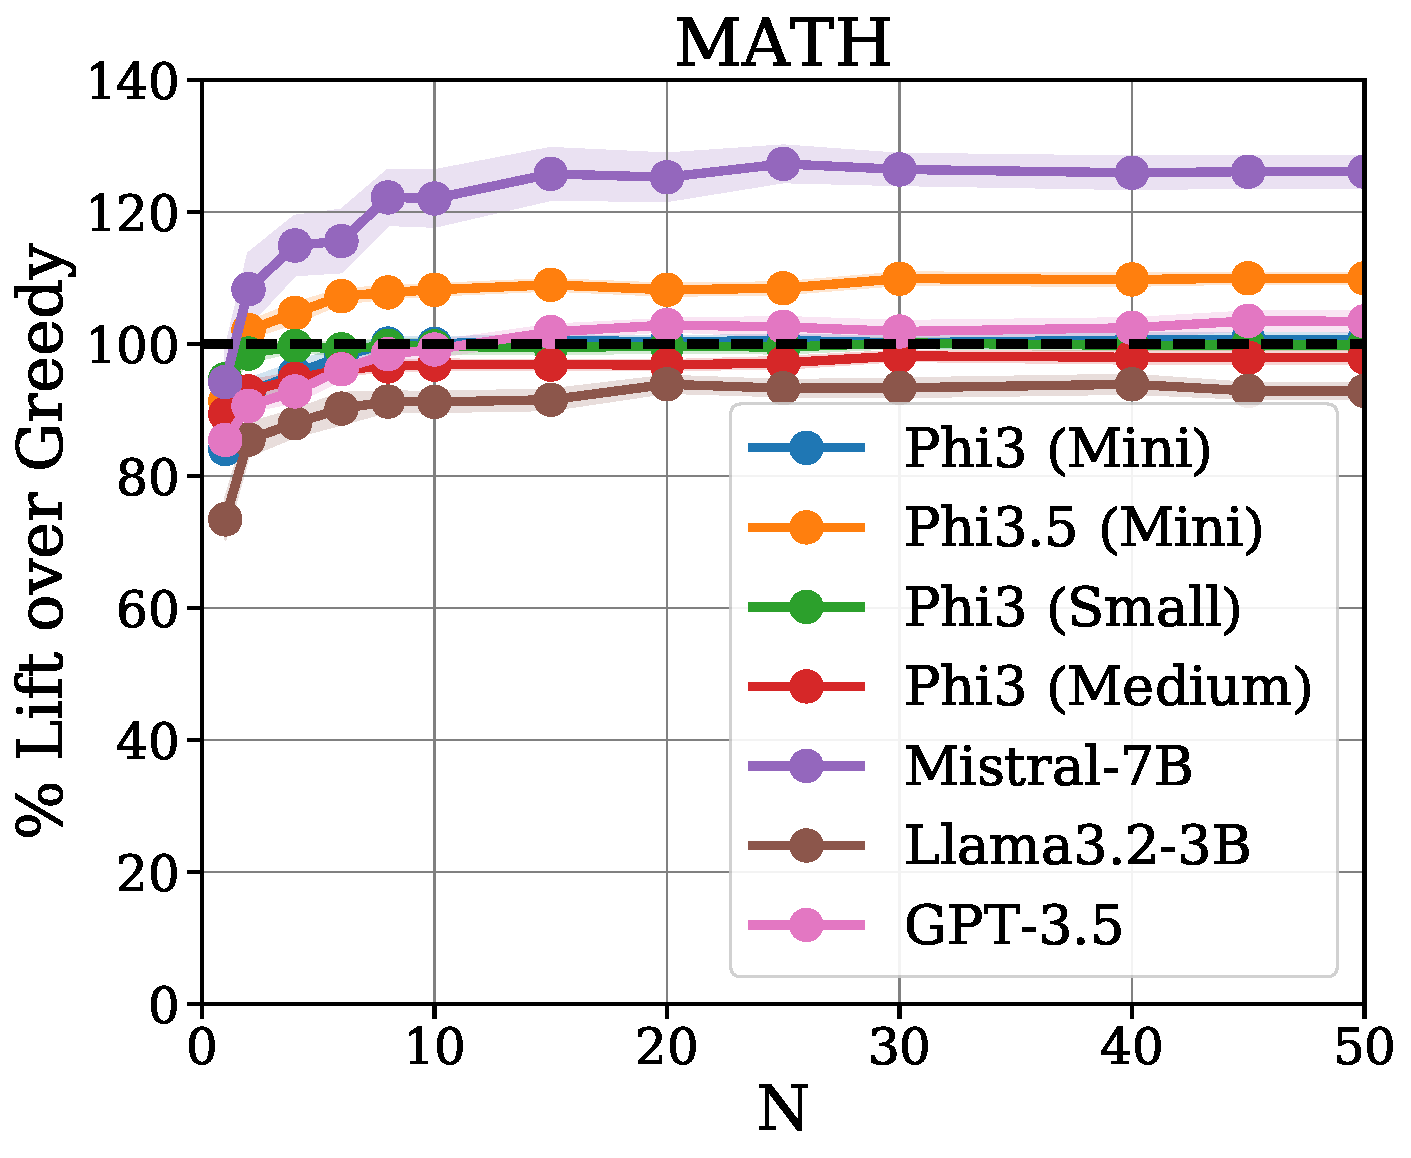
\includegraphics[width=0.28\textwidth]{figs/BoN-math-improvement.pdf}
        \label{sfig:bon-math-improvement}
    }
    \hfill
    \subfigure[]{
        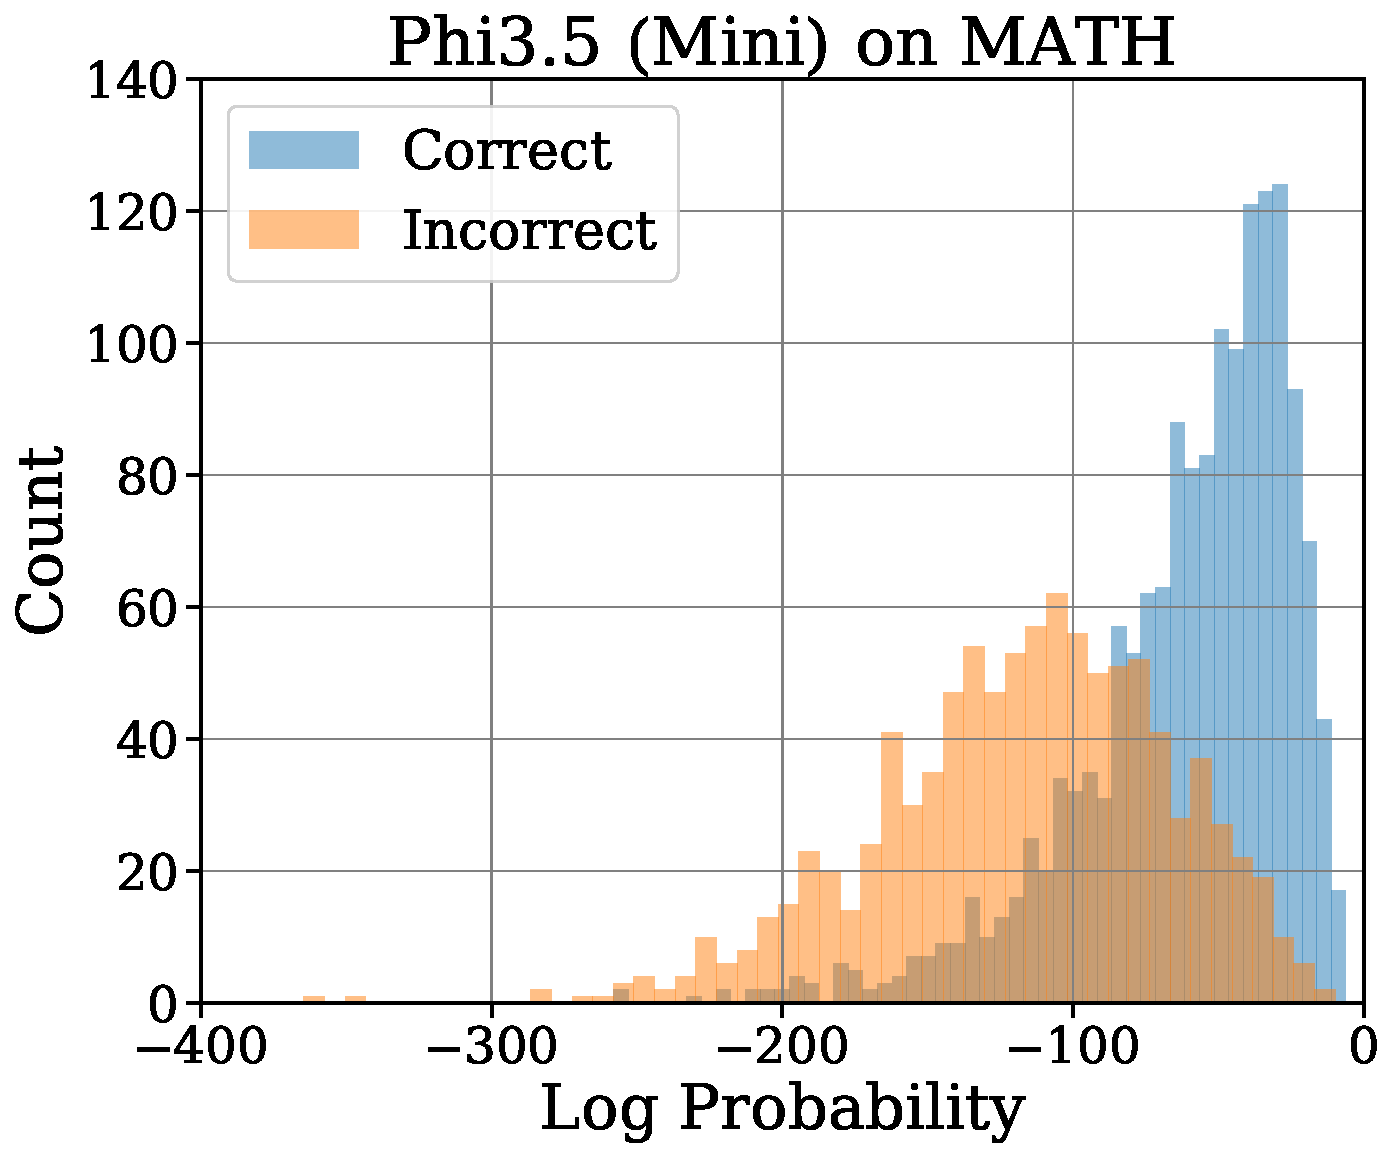
\includegraphics[width=0.28\textwidth]{figs/Logprob-Distribution-phi35mini-math.pdf}
        \label{sfig:logprob-sitribution}
    }
    \vspace{-0.25cm}
    \caption{Validation of maximum-likelihood sharpening, via
      Best-of-$N$ (BoN) sampling, at inference time. (a) Percent
      accuracy improvement over greedy decoding for BoN sharpening
      with $N=50$ on 6 tasks and 7 models, colored by performance.
      (b) Perecent accuracy improvement over greedy for BoN sharpening as a
      function of $N$ for 7 different models on the MATH dataset.  (c)
      Distribution over sequence-level log probabilities for sampled
      completions ($N=1$) from \phithreefivemini on the MATH dataset,
      conditioned on whether or not the completion is correct.
      Correct completions are noticeably in higher likelihood than incorrect completions, demonstrating the utility of inference-time sharpening.}\label{fig:validation}\vspace{-0.25cm}
\end{figure}




In this paper, we posit a potential source of hidden knowledge, and
offer a formal perspective on how
to extract it. %
Our starting point is the widely observed phenomenon that language models are often better at verifying whether
responses are correct than they are at generating correct
responses \citep{huang2022large,wang2022self,bai2022constitutional,pang2023language,yuan2024self}. %
This gap may be explained by the theory of computational complexity, which suggests that generating high-quality
responses can be less computationally tractable than verification
\citep{cook1971complexity,levin1973universal,karp1972reducibility}. In
autoregressive language modeling, computing the most likely response for a given
prompt is $\NP$-hard in the worst case (\cref{sec:hardness}), whereas the model's likelihood for
a given response can be easily evaluated.\looseness=-1


We view self-improvement as any attempt to narrow this gap, i.e., use the model as its own
verifier to improve generation and \emph{sharpen} the model toward
  high-quality responses.
Formally, consider a learner with access to a base model
$\piref:\cX\to\Delta(\cY)$ representing a conditional distribution
that maps a prompt $x\in\cX$ to a distribution over responses
(i.e., $\piref(y\mid{}x)$ is the probability that the model generates
the response $y$ given the prompt $x$).\iclr{\footnote{Our \arxiv{most }general results are
agnostic to the structure of $\cX$, $\cY$, and $\piref$, but an
important special case for language modeling is the autoregressive setting where
$\cY=\cV^{H}$ for a vocabulary space $\cV$ and sequence
  length $H$, and where $\piref$ has the autoregressive structure
$\piref(y_{1:H}\mid{}x)=\prod_{h=1}^{H}\pirefh(y_h\mid{}y_{1:h-1},x)$
for $y=y_{1:H}\in\cY$.\loose}} 
We posit that $\piref$ has already been trained in some manner
  (e.g., through next-token prediction or additional post-training steps such as SFT or RLHF), 
with the key feature being that $\piref$ is a good verifier, as measured by some \emph{self-reward} function $\rself (y \mid x; \piref)$ measuring model certainty.
The self-reward
function is derived purely from the base model $\piref$, without external supervision or feedback. Examples include
normalized and/or regularized sequence likelihood \citep{meister2020if}, models-as-judges \citep{zheng2024judging,yuan2024self,wu2024meta,wang2024self}, and model
confidence \citep{wang2024chain}.\loose



\begin{tcolorbox}[enhanced,title=Sharpening,
    colframe=blue!40!black,
    colback=blue!2!white,
    fonttitle=\bfseries,
  attach boxed title to top text left={xshift=30mm,yshift=-2.5mm},
  boxed title style={size=small,colframe=blue!40!black,colback=blue!40!black}]
    We refer to \textbf{sharpening} as any process that tilts $\piref$
  toward responses that are more certain in the sense that they
  enjoy greater self-reward $\rself$.
  That is, a sharpened model $\pihat$ is one that
  (approximately) maximizes the self-reward:
  \loose
  \begin{align}
    \label{eq:sharpening}
    \pihat(x)\approx \argmax_{y\in\cY}\rself(y\mid{}x; \piref).
  \end{align}
\end{tcolorbox}
            
        
\akdelete{Note that, in \cref{eq:sharpening}, $y$ denotes an entire response, rather than a single token.
Sharpening may be implemented at inference-time, or \textbf{amortized} via
self-training (\Cref{sec:algorithms}). Popular decoding
strategies such as greedy, low-temperature sampling, and beam-search can all be
viewed as instances of the former (albeit at the
token-level).\footnote{More sophisticated decoding strategies like
normalized/regularized sequence likelihood
\citep{meister2020if} or chain-of-thought decoding
\citep{wang2024chain} \iclr{\abedit{also} admit an interpretation as sharpening;
see \cref{sec:additional_related}.}\arxiv{use various metrics of model
``confidence'' to guide sampling in the
  absence of external verifiers; these too admit an informal
  interpretation as ``sharpening''. See \cref{sec:additional_related}.}\loose}
The latter captures many existing self-training schemes
\citep{huang2022large,wang2022self,bai2022constitutional,pang2023language,yuan2024self},
and is the main focus of this paper; we use the term \emph{sharpening} without further qualification to
  refer to the latter.\loose}



\akedit{An important special case for sharpening is in
  language/autoregressive modeling. Here, we have $\cY = \cV^H$ for a
  vocabulary space $\cV$ and sequence length $H$, and $\piref$ has the
  autoregressive structure $\piref(y_{1:H}\mid{}x) = \prod_{h=1}^H
  \pirefh(y_h \mid{}y_{1:h-1},x)$ for $y = y_{1:H} \in
  \cY$. Sharpening in this setting pertains to entire responses, i.e.,
  the optimization over responses in \Cref{eq:sharpening} is at the \emph{sequence level}. In contrast, popular decoding strategies such as greedy, low-temperature sampling, and beam search operate at the token-level; nevertheless, they can be viewed as heuristics for \emph{inference-time sharpening}.\footnote{More sophisticated decoding strategies like
normalized/regularized sequence likelihood
\citep{meister2020if} or chain-of-thought decoding
\citep{wang2024chain} \iclr{\abedit{also} admit an interpretation as sharpening;
see \cref{sec:additional_related}.}\arxiv{use various metrics of model
``confidence'' to guide sampling in the
  absence of external verifiers; these too admit an informal
  interpretation as ``sharpening''. See \cref{sec:additional_related}.}\loose} The combinatorial response space can make sharpening computationally demanding and so, an appealing alternative to inference-time sharpening is \emph{amortization via self-training} (\Cref{sec:algorithms}). The latter captures many existing self-training schemes
\citep{huang2022large,wang2022self,bai2022constitutional,pang2023language,yuan2024self},
and is the main focus of this paper; we use the term \emph{sharpening} without further qualification to
  refer to the latter.\loose}

We refer to the \textbf{sharpening mechanism} as the phenomenon where responses from a model with the highest certainty (in the sense
of large self-reward $\rself$) exhibit the greatest performance on a
task of interest. Though it is unclear a-priori whether there are self-rewards related to task performance, the successes of self-improvement in prior works \citep{huang2022large,wang2022self,bai2022constitutional,pang2023language,yuan2024self} give strong positive evidence.
These works suggest that, in many settings, models do have hidden knowledge: the model's own self-reward correlates with response quality, but it is computationally challenging to generate high self-rewarding---and thus high quality---responses. It is the role of (algorithmic) sharpening to leverage these verifications to improve the quality of generations, despite computational difficulty.\loose






        
        












        
        
\newcommand{\rbase}{r_{\mathrm{base}}}












    





    
    

    





    
            
    

    


    





\subsection{Contributions}





We initiate the theoretical study of self-improvement via the
sharpening mechanism. We disentangle the choice of self-reward from the algorithms used to optimize it, and aim to
understand: (i) When and how does self-training
achieve sharpening? (ii) What are the fundamental
limits for self-training algorithms?\loose
\arxiv{\dfc{above seems like the most clear description of what we do, but it
  would be nice if we could also weave in experiments.}}

\paragraph{Algorithms for sharpening (\cref{sec:algorithms})}
The starting point for our work is to consider
two natural families of self-improvement algorithms based on
supervised fine-tuning (SFT) and reinforcement learning (RL/RLHF),
respectively, \bestofnalg and \rlhfalg. Both algorithms \textbf{amortize} the
sharpening objective \eqref{eq:sharpening} into a dedicated
post-training/fine-tuning phase:
\begin{itemize}
\item \bestofnalg filters responses where the self-reward $\rself(y\mid{}x;\piref)$
  is large and fine-tunes on the resulting dataset, invoking common
  SFT pipelines
\arxiv{\citep{amini2024variational,sessa2024bond,gui2024bonbon,pace2024west}}\iclr{\citep{amini2024variational,sessa2024bond}}.\loose
  \item \rlhfalg{} directly applies reinforcement learning techniques (e.g.,
  PPO~\citep{schulman2017proximal} or DPO~\citep{rafailov2024direct}) to optimize the self-reward function $\rself(y\mid{}x;\piref)$.
\end{itemize}
In the remainder of the paper, we introduce a theoretical framework to analyze the performance of these
  algorithms\iclr{.}\arxiv{, and validate our findings empirically.} Our main contributions are as follows.



\paragraph{Maximum-likelihood sharpening objective
  (\Cref{sec:autoreg_sharpening})} As a concrete proposal for one
source of hidden knowledge, we focus on self-rewards defined by the model's sequence-level log-probabilities:
\begin{align}
  \label{eq:ml_sharpening}
    \rself(y \mid x; \piref) := \log \piref(y \mid x)
\end{align}
This is a 
stylized self-reward function, which offers perhaps the simplest objective for
self-improvement in the absence of external feedback (i.e., purely
supervision-free), yet also connects self-improvement to a rich body of theoretical computer science literature on computational trade-offs for optimization (inference) versus sampling (\Cref{sec:additional_related}). 
\arxiv{\akedit{We view \Cref{eq:ml_sharpening} as a \emph{clean and minimal objective} that reveals the interplay between hidden knowledge, computational bottlenecks, and self-improvement in generative model.}}
In spite of its simplicity,\arxiv{ we show empirically
that} \mlsharp is already sufficient to achieve non-trivial performance gains \akedit{over greedy decoding on a range of 
reasoning tasks with several language models;}\akdelete{reasoning tasks such as \gametwentyfour, \gsm, and \mathdataset \abedit{over greedy decoding};} cf. \cref{fig:validation}. We believe it can serve as a starting point toward
understanding forms of self-improvement that use more
sophisticated self-rewarding\arxiv{ or judging but are less amenable to theoretical analysis}
\citep{huang2022large,wang2022self,\arxiv{bai2022constitutional,}pang2023language,yuan2024self}. \loose














  
  

















        


      

\paragraph{A statistical framework for sharpening
(\cref{sec:sample,sec:lower})} Though the goal of sharpening is
computational in nature, we recast self-training according to the
\mlsharp objective \cref{eq:ml_sharpening} as
a \textbf{statistical} problem where we aim to produce a model
approximating \eqref{eq:sharpening} using a polynomial number of (i)
sample prompts $x \sim \mu$, (ii) sampling queries of the form $y
\sim \piref(x)$, and (iii) likelihood evaluations of the form $\piref(y \mid x)$. 
\iclr{Evaluating the efficiency of the algorithm through the number of such queries, this abstraction
offers a natural way to evaluate the performance of self-improvement/sharpening
algorithms and establish fundamental limits; we use our framework to prove new
lower bounds that highlight the importance of
the base model's coverage.
}
\arxiv{Evaluating the efficiency of the algorithm through the number of such queries, this abstraction
offers a natural way to evaluate the performance of self-improvement/sharpening
algorithms and establish fundamental limits and minimax optimality,
similar to the role of information-based complexity in optimization
\citep{nemirovski1983problem,traub1988information,raginsky2011information,agarwal2012information}, 
statistical query complexity in computational learning theory
\citep{blum1994weakly,kearns1998efficient,feldman2012complete,feldman2017general},
and query complexity more broadly. We use our framework to prove new
lower bounds and fundamental limits which highlight the importance of \abedit{the base model's}
\emph{coverage} (that is, probability mass placed on high-quality responses). 
}





\paragraph{Analysis of sharpening algorithms (\cref{sec:theoretical_analysis})}
Within our statistical framework for \arxiv{maximum-likelihood }sharpening, we show that
\bestofnalg and \rlhfalg provably converge to sharpened models,
establishing several results:\iclr{ \textbf{(i) \bestofnalg is
    minimax optimal}, and learns a sharpened model whenever $\piref$ has
  sufficient coverage (we also show
  that a novel variant based on adaptive sampling can sidestep
  the minimax lower bound); \textbf{(ii) \rlhfalg benefits from
    on-policy exploration}, and can bypass
  the need for coverage---improving over \bestofnalg.\loose
  }
\arxiv{\begin{itemize}
\item \textbf{Optimality of \bestofnalg.} We show that \bestofnalg
  succeeds at learning a sharpened model whenever $\piref$ has
  sufficient coverage, and is minimax
  optimal in a worst-case sense. Perhaps surprisingly, we show
  that a novel variant based on adaptive sampling can bypass
  this lower bound.
\item \textbf{Benefits of \rlhfalg.} We show that \rlhfalg
  also succeeds at learning a sharpened model and achieves similar performance to \bestofnalg when $\piref$ has
  sufficient coverage. However, we show that this algorithm can bypass
  the need for coverage---improving over \bestofnalg---by leveraging
  deliberate \emph{exploration} of the response space.\loose
\end{itemize}
}
\paragraph{Empirical investigation (\Cref{sec:experiments})}  We
empirically explore the extent to which our theoretical framework can aid language models in a variety of tasks.  We first consider three choices of self-reward, including \mlsharp, and sharpen via a practical approximation, inference-time best-of-N sampling: given a prompt $x \in \cX$, we draw $N$ responses $y_1,\ldots,y_N\sim\piref(\cdot\mid{}x)$ and return the response $\widehat{y} = \argmax_{y_i} \rself(y_i \mid{}x)$; this is
equivalent to \iftoggle{workshop}{\cite{stiennon2020learning,gao2023scaling,yang2024asymptotics}}{\citet{stiennon2020learning,gao2023scaling,yang2024asymptotics}} \abedit{and is a popular approach in modern deployments}.\footnote{We mention in passing that
  inference-time \bestofn sampling enjoys provable guarantees for
  maximizing the \mlsharp objective when $N$ is sufficiently
  large. See \cref{sec:inference} for details.}
We consider an extensive list of model-dataset pairs and find that sharpening, even with the stylized maximum-likelihood self-reward, often improves performance over greedy decoding. 
  We then implement one of our algorithms, \bestofnalg, on a subset of
  these model-dataset pairs and observe a significant positive effect
  on performance, indicating that sharpening can indeed be amortized.  An overview of our inference-time experiments can be found in \Cref{fig:validation}.


\dfc{Feels like we should perhaps advertise the fact that we are doing
  this in a learning-theoretic way that abstracts away the role of
  optimization/model and allows for general function classes. For
  arxiv I think we should definitely add a paragraph about this at least.
  }













  
\subsection{Related Work}

Our work is most directly related to a growing body of empirical research that
studies self-training for language models in a
supervision-free setting with no external
feedback~\citep{huang2022large,wang2022self,bai2022constitutional,pang2023language,yuan2024self}.
The
specific algorithms for self-improvement/sharpening we study can be
viewed as applications of standard alignment algorithms
\citep{amini2024variational,sessa2024bond,\arxiv{gui2024bonbon,pace2024west,}christiano2017deep,bai2022training,ouyang2022training,rafailov2024direct}
with a specific choice of reward function. 
However, the maximum
likelihood sharpening objective \eqref{eq:ml_sharpening} used for our
theoretical results has been relatively unexplored within the
alignment and self-improvement literature.\loose

\dfc{Add yuda's paper once it's online.}


      On the theoretical side, current understanding of self-training is limited. One line of work, focusing on the
      \emph{self-distillation} objective \citep{hinton2015distilling}
      for classification and regression, aims to provide convergence
      guarantees for self-training in stylized setups such as linear
      models
      \citep{mobahi2020self,frei2022self,das2023understanding,das2024retraining,pareek2024understanding},
      with 
      \iftoggle{workshop}{\cite{allen2020towards}}{\citet{allen2020towards}} giving guarantees for feedforward
      neural networks and \citet{boix2024towards} proposing a general
      PAC-style framework. 
      To the best of our knowledge, our work is the first to study
      self-training in a general framework that subsumes language
      modeling. \iclr{See \cref{sec:additional_related} for a more extensive discussion of
        related work.\loose}
      


     

\arxiv{See \cref{sec:additional_related} for a more extensive discussion of
related work.} 

\arxiv{
\paragraph{Notation}
  For an integer $n\in\bbN$, we let $[n]$ denote the set
  $\{1,\dots,n\}$. For a set $\cX$, we let $\Delta(\cX)$ denote the
  set of all probability distributions over $\cX$. We adopt
    standard big-oh notation, and write $f=\bigoht(g)$ to denote that
    $f = \bigoh(g\cdot{}\max\crl*{1,\mathrm{polylog}(g)})$,
    $a\approxleq{}b$ as shorthand for $a=\bigoh(b)$, and $a \asymp{} b$ as shorthand for $a = \Theta(b)$. \loose
    }









